\let\negmedspace\undefined
\let\negthickspace\undefined
\documentclass[journal]{IEEEtran}
\usepackage[a5paper, margin=10mm, onecolumn]{geometry}
\usepackage{tfrupee} 

\setlength{\headheight}{1cm}
\setlength{\headsep}{0mm}

\usepackage{gvv-book}
\usepackage{gvv}
\usepackage{cite}
\usepackage{amsmath,amssymb,amsfonts,amsthm}
\usepackage{algorithmic}
\usepackage{graphicx}
\usepackage{textcomp}
\usepackage{xcolor}
\usepackage{txfonts}
\usepackage{listings}
\usepackage{enumitem}
\usepackage{mathtools}
\usepackage{gensymb}
\usepackage{comment}
\usepackage[breaklinks=true]{hyperref}
\usepackage{tkz-euclide} 
\usepackage{listings}

\def\inputGnumericTable{}                                 
\usepackage[latin1]{inputenc}                                
\usepackage{color}                                            
\usepackage{array}                                            
\usepackage{longtable}                                       
\usepackage{calc}                                             
\usepackage{multirow}                                         
\usepackage{hhline}                                           
\usepackage{ifthen}                                           
\usepackage{lscape}

\title{\textbf{2.7.18}}
\author{\textbf{EE25BTECH11006 - ADUDOTLA SRIVIDYA}}
\date{september 11, 2025}

\begin{document}

\maketitle

Question:\\
Vertices of a $\triangle ABC$ are $\vec{A}(4,6)$, $\vec{B}(1,5)$ and $\vec{C}(7,2)$.  
A line segment $DE$ is drawn intersecting AB and AC at D and E respectively such that  
$\dfrac{AD}{AB} = \dfrac{AE}{AC} = \dfrac{1}{3}$.  
Calculate the area of $\triangle ADE$ and compare it with the area of $\triangle ABC$.\\

\solution\\
Let
\begin{align}
    \vec{A} &= \myvec{4\\6}, \quad
    \vec{B} = \myvec{1\\5}, \quad
    \vec{C} = \myvec{7\\2}
\end{align}

Point $\vec{D}$ divides $AB$ in ratio $1:2$:
\begin{align}
    \vec{D} &= \frac{2\vec{A} + 1\vec{B}}{3} 
             = \frac{2\myvec{4\\6} + \myvec{1\\5}}{3} 
             = \myvec{3\\\tfrac{17}{3}}
\end{align}

Point $\vec{E}$ divides $AC$ in ratio $1:2$:
\begin{align}
    \vec{E} &= \frac{2\vec{A} + 1\vec{C}}{3} 
             = \frac{2\myvec{4\\6} + \myvec{7\\2}}{3} 
             = \myvec{5\\\tfrac{14}{3}}
\end{align}

Area of a triangle with vertices $\vec{P}, \vec{Q}, \vec{R}$ is
\begin{align}
    \Delta &= \tfrac{1}{2}\Bigg|\det \myvec{x_Q - x_P & x_R - x_P \\ y_Q - y_P & y_R - y_P}\Bigg|
\end{align}

So,
\begin{align}
    \Delta_{ABC} &= \tfrac{1}{2}\left|\det \myvec{1-4 & 7-4 \\ 5-6 & 2-6}\right| \\
                 &= \tfrac{1}{2}\left|\det \myvec{-3 & 3 \\ -1 & -4}\right| \\
                 &= \tfrac{1}{2}(12+3) \\
                 &= \tfrac{15}{2}
\end{align}

Similarly,
\begin{align}
    \Delta_{ADE} &= \tfrac{1}{2}\left|\det \myvec{3-4 & 5-4 \\ \tfrac{17}{3}-6 & \tfrac{14}{3}-6}\right| \\
                 &= \tfrac{1}{2}\left|\det \myvec{-1 & 1 \\ -\tfrac{1}{3} & -\tfrac{4}{3}}\right| \\
                 &= \tfrac{1}{2}\left(\tfrac{4}{3}+\tfrac{1}{3}\right) \\
                 &= \tfrac{5}{6}
\end{align}

Thus,
\begin{align}
    \frac{\Delta_{ADE}}{\Delta_{ABC}}
    &= \frac{\tfrac{5}{6}}{\tfrac{15}{2}}
     = \frac{1}{9}
\end{align}

Therefore,
\begin{align}
    \text{Area of } \triangle ADE = \tfrac{1}{9} \text{ of area of } \triangle ABC.
\end{align}

\begin{figure}[H]
    \centering
    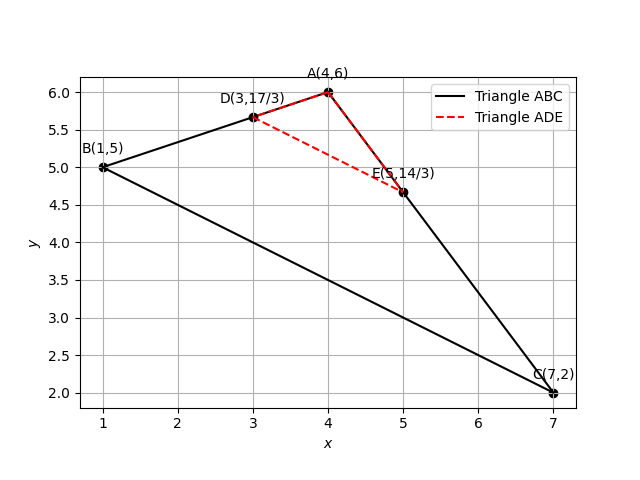
\includegraphics[width=0.6\linewidth]{figs/fig4.png}
    \caption{Triangle ABC with inner triangle ADE}
    \label{fig:1}
\end{figure}

\end{document}